%----------------------------------------------------------
\def\notedate{2023.03.30}
\def\currentauthor{Василян А.Р. (РК6-83Б)}
%----------------------------------------------------------
\notestatement{rndhpcgui}{Генерация страницы на основе данных в формате aINI.}

%---------------------------------------------------------
Была улучшена программа преобразования кода \textsf{aINI} в \textsf{HTML}-код. Теперь сегменты реализованы не как заголовки, а как вкладки на странице, между которыми  можно переходить по нажатию.

Содержимое каждого сегмента записывается последовательно в один элемент списка \textsf{elements_list}, а сам сегменты хранятся в списке \textsf{sections_list}.  

Создаются кнопки для открытия содержимого определенной вкладки. Все элементы \textsf{<div>} с классом \textsf{tabcontent} скрыты по умолчанию (с помощью \textsf{CSS} (\ref{rndhpcgui.2023.03.30.css}) и \textsf{JS} (~\ref{rndhpcgui.2023.03.30.js})). Когда пользователь нажимает на кнопку - открывается содержимое вкладки, которое соответствует этой кнопке.


\begin{lstlisting}[frame=single, label={rndhpcgui.2023.03.30.css}, caption={CSS стили}, language={HTML}] 
    /* стиль вкладки */
    .tab {
        overflow: hidden;
        border: 1px solid #ccc;
        background-color: #f1f1f1;
    }
    
    /* стиль кнопки вкладки */
    .tab button {
        background-color: inherit;
        float: left;border: none;
        outline: none;
        cursor: pointer;
        padding: 14px 16px;
        transition: 0.3s;
        font-size: 17px;
    }
    
    /* Измените цвет фона кнопок при наведении курсора мыши */
    .tab button:hover {
        background-color: #ddd;
    }
    
    /* класс текущей/активной вкладки */
    .tab button.active {
        background-color: #ccc;
    }
    
    /* стиль содержимого вкладки */
    .tabcontent {
        display: none;
        padding: 6px 12px;
        border: 1px solid #ccc;
        border-top: none;
    }
    
    /* стиль закрывающей кнопки */
    .topright {
        float: right;
        cursor: pointer;
        font-size: 28px;
    }
    
    .topright:hover {color: red;}
\end{lstlisting}


Получение всех элементов с классом \textsf{tabcontent} и скрытие их (\ref{rndhpcgui.2023.03.30.js1}).

\begin{lstlisting}[frame=single, label={rndhpcgui.2023.03.30.js1}, caption={JavaScript код скрытия вкладок}, language={HTML}]
    tabcontent = document.getElementsByClassName("tabcontent");
    for (i = 0; i < tabcontent.length; i++) {
        tabcontent[i].style.display = "none";
    }
\end{lstlisting}


Получение всех элементов с классом \textsf{tablinks} и удаления у них класса \textsf{active} (\ref{rndhpcgui.2023.03.30.js2}).

\begin{lstlisting}[frame=single, label={rndhpcgui.2023.03.30.js2}, caption={JavaScript код удаления класса \textsf{active}}, language={HTML}]
    tablinks = document.getElementsByClassName("tablinks");
    for (i = 0; i < tablinks.length; i++) {
        tablinks[i].className = tablinks[i].className.replace(" active", "");
    }
\end{lstlisting}

Изображение текущей вкладки и добавление класса \textsf{active} кнопке, открывающую эту вкладку (\ref{rndhpcgui.2023.03.30.js3}).

\begin{lstlisting}[frame=single, label={rndhpcgui.2023.03.30.js3}, caption={JavaScript код изображения текущей вкладки}, language={HTML}]
    document.getElementById(tab_id).style.display = "block";
    evt.currentTarget.className += " active";
\end{lstlisting}


Функция \textsf{tabs} (\ref{rndhpcgui.2023.03.30.js}) вызывается при событии \textsf{onclick} (нажатие) у элементов кнопок вкладок, например \ref{rndhpcgui.2023.03.30.tab_button}.

\begin{lstlisting}[frame=single, label={rndhpcgui.2023.03.30.tab_button}, caption={Элементы кнопок вкладок}, language={HTML}] 
<div class="tab">
	<button class="tablinks" onclick="tabs(event,'section_0')" id="defaultOpen">Пункт 1</button>
	<button class="tablinks" onclick="tabs(event,'section_1')">Пункт 2</button>
</div>
\end{lstlisting}


\begin{lstlisting}[frame=single, label={rndhpcgui.2023.03.30.js}, caption={полный JavaScript код}, language={HTML}] 
    <script>
    function tabs(evt, tab_id) {
        var i, tabcontent, tablinks;
        tabcontent = document.getElementsByClassName("tabcontent");
        for (i = 0; i < tabcontent.length; i++) {
            tabcontent[i].style.display = "none";
        }
        tablinks = document.getElementsByClassName("tablinks");
        for (i = 0; i < tablinks.length; i++) {
            tablinks[i].className = tablinks[i].className.replace(" active", "");
        }
        document.getElementById(tab_id).style.display = "block";
        evt.currentTarget.className += " active";
    }
    
    document.getElementById("defaultOpen").click();
    </script>
\end{lstlisting}

Пример сгенерированной страницы в запущенном web-приложении на рисунках~\ref{rndhpcgui.2023.03.30.picture1} и~\ref{rndhpcgui.2023.03.30.picture2}.
\begin{figure}[!ht]
  \centering
  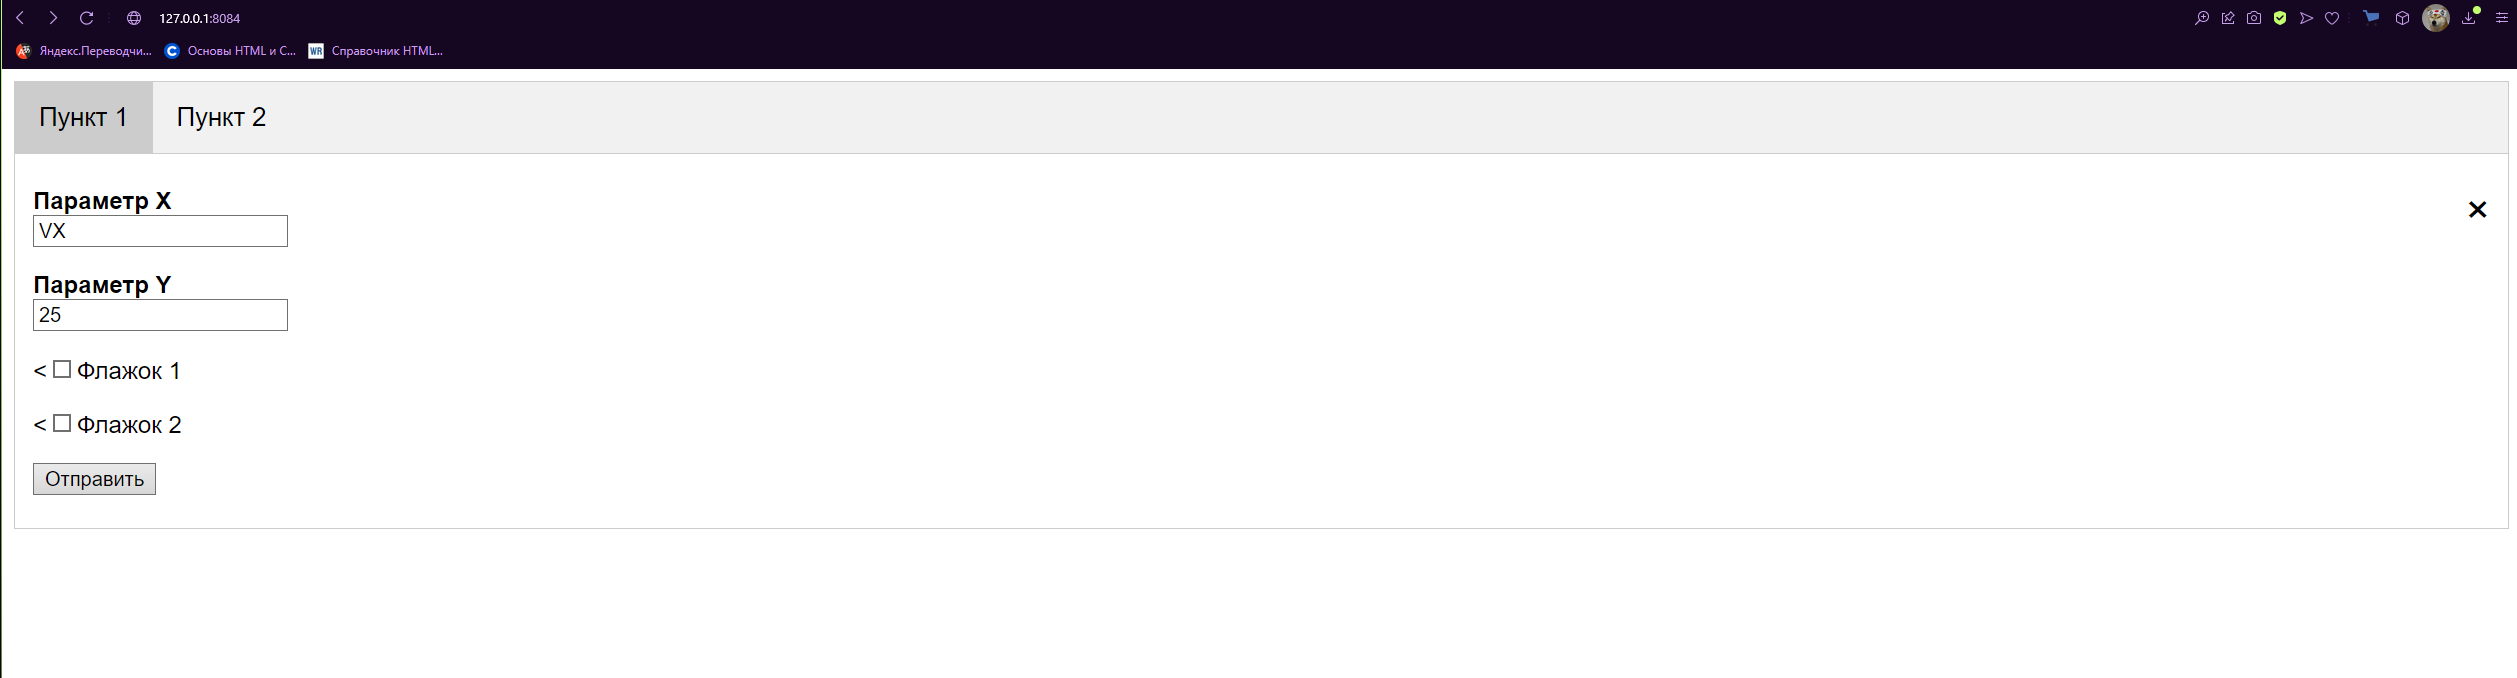
\includegraphics[scale=0.4]{ResearchNotes/rndhpc_dev_gui_2023_03_30/rndhpcgui.2023.03.30.picture1.png}
  \caption{Пример}
  \label{rndhpcgui.2023.03.30.picture1}
\end{figure}

\begin{figure}[!ht]
    \centering
    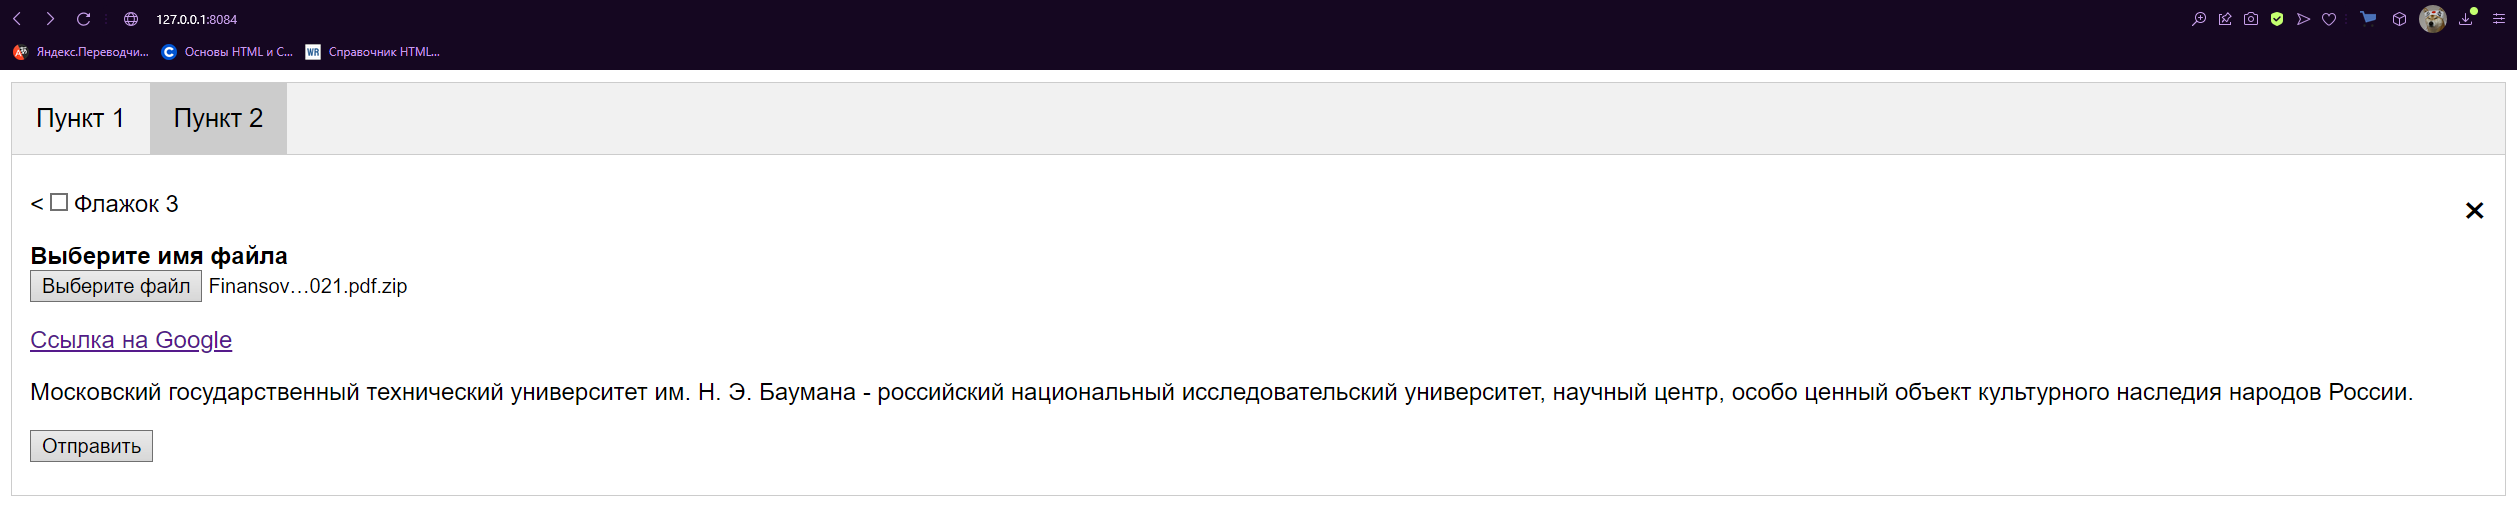
\includegraphics[scale=0.4]{ResearchNotes/rndhpc_dev_gui_2023_03_30/rndhpcgui.2023.03.30.picture2.png}
    \caption{Пример}
    \label{rndhpcgui.2023.03.30.picture2}
  \end{figure}
%----------------------------------------------------------
% Атрибуты задачи
\noteattributes{}
%----------------------------------------------------------
